\section{Figure Construction and Additional Examples}
\label{app:visual-examples}
\subsection{Construction of the Main-Text Displays}
Figure~\ref{fig:elvis-example} uses 32 grayscale contours selected inside
an annotated foreground region, plus photo-guided paths for the outer pose,
microphone and cable. Curve weights are proportional to arclength, occupancy
is uniform in normalized arclength, and kernel covariance is $0.014^2I_2$.
The 18,000 draws use seed 2026102205. Its density display uses 4096 midpoint
nodes per curve, a $500\times500$ grid and Gaussian convolution. Coordinates
are scaled image-plane coordinates; photographic brightness does not set
component mass.

Figure~\ref{fig:volcano} uses the circular-tube law specified in the main
text, with 16,000 draws and seed 2026102206. Its $64\times64$ bivariate
histogram displays $[-2.25,2.25]^2$, containing 15,853 observations; the
remaining 147 draws are outside this window. Bin density divides by the
full sample size and bin area. All radii enter the lower histogram.
Figure~\ref{fig:fermat-section} uses 18,000 draws and seed 2026102207
from the finite-curve law in Appendix~\ref{app:fermat-construction}.

Figure~\ref{fig:reference-histograms} uses the first two coordinates of
a ten-dimensional correlated Gaussian, a ten-dimensional skew mixture and
a two-dimensional banana transform. All 500 stored training observations
from repetition~1 of each reference scenario enter the histograms. The
$24\times24$ joint bin densities use count divided by sample size and bin
area and integrate to one. The lower panels are first-coordinate marginals.

\subsection{Three-Dimensional and Other Specified Laws}
Figure~\ref{fig:face-example} shows a three-dimensional law, retaining its
third-coordinate observations. Its localized Gaussian components have
positive covariance, whereas an exact atom in Definition~\ref{def:sfd}
is a point mass. The main-text density surfaces in
Figure~\ref{fig:density-examples} use the first two coordinates instead.
Their displayed heights are proportional to $(p/\max p)^a$, with
panel-specific exponents $a=0.28,0.1664,0.36,0.36$ for the snowflake,
face, maze and ECG-like laws. Colors also use panel-specific nonlinear
relative scales. The face uses tube SD 0.070 and blob SD 0.105, different
from the narrower sample illustration below. These displays are specified
laws, without fitted-method comparisons.

\begin{figure}[t]
\centering
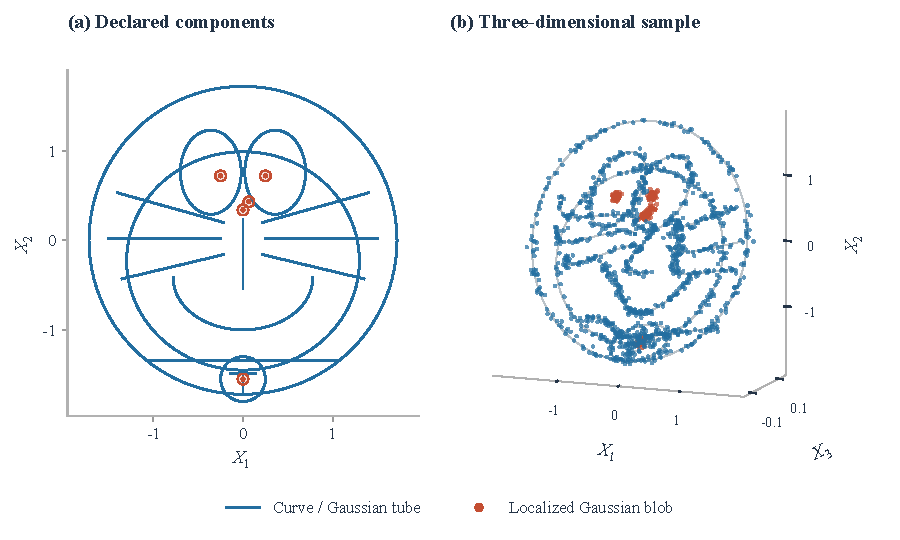
\includegraphics[width=0.93\linewidth,clip]{figures/face_example_3d.pdf}
\caption{A stylized-face SFD with 16 Gaussian tubes and five localized
Gaussian components. Left: projected centerlines and blob contours at
squared Mahalanobis distance four. Right: all 1,600 observations in three
dimensions, with gray centerlines as guides. Blue and red identify tubes
and blobs. Branch coordinates are uniform on $[0,1]$; SDs in the first two
coordinates are 0.020 for tubes and 0.030 for blobs, and the
third-coordinate SD is 0.012. The right panel uses actual $X_3$ values with
unequal display scales.}
\label{fig:face-example}
\end{figure}

\FloatBarrier
